% !TEX root = thesis.tex

\section{Results}\label{sec:results}
\renewcommand{\thefigure}{\thesection.\arabic{figure}}
\begin{figure*}
  \centering
  \begin{subfigure}[b]{0.3\textwidth}
    \centering
    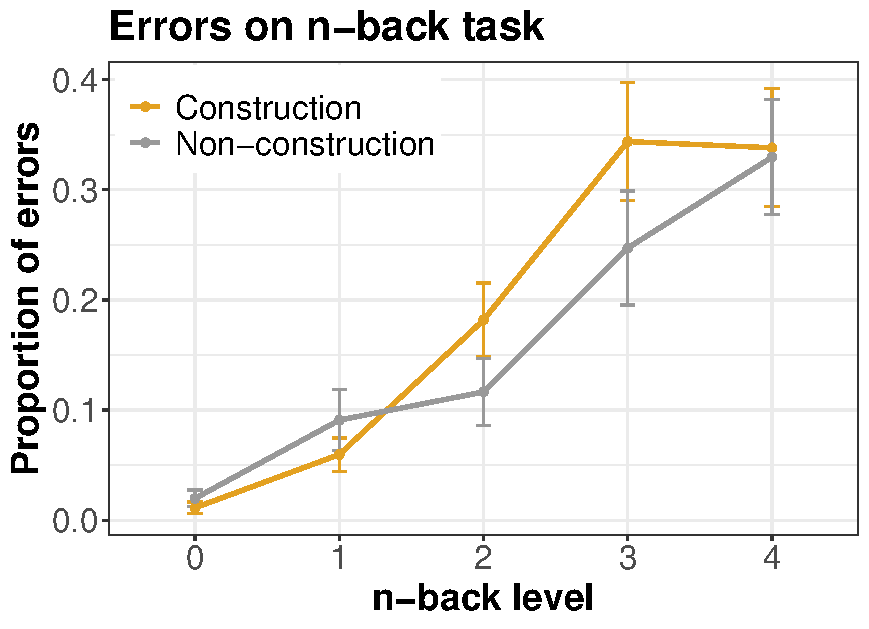
\includegraphics[width=\textwidth]{images/error_rates.pdf}
    \caption{Errors on the \textit{n}-back task (\textit{N}\ =\ 22). From \citet{DeMooij2021}.}
    \label{fig:errors}
  \end{subfigure}
  \hfill
  \begin{subfigure}[b]{0.3\textwidth}
    \centering
    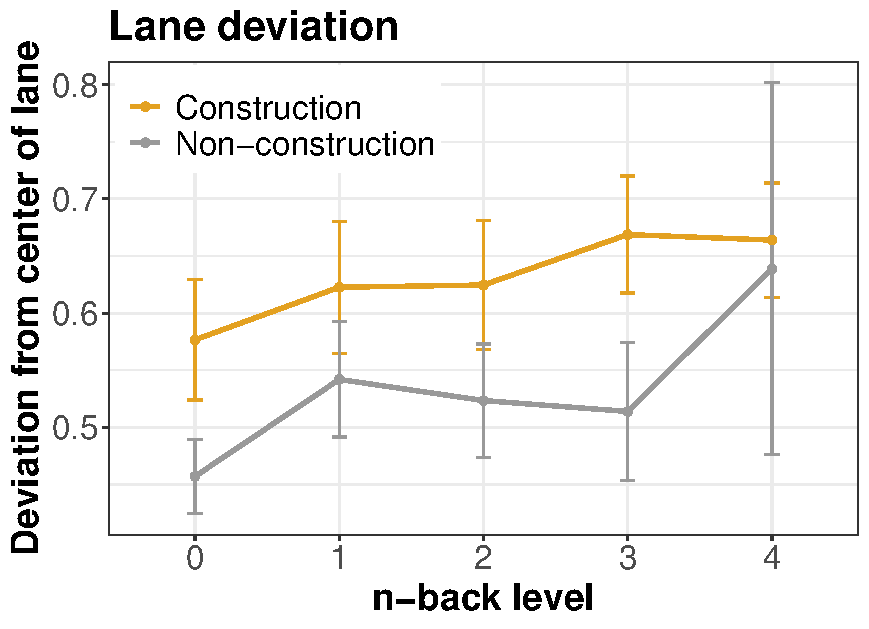
\includegraphics[width=\textwidth]{images/lane_deviation.pdf}
    \caption{Lane deviation (\textit{N}\ =\ 22). From \citet{Kelapanda2021}.}
    \label{fig:lane-deviation}
  \end{subfigure}
  \hfill
  \begin{subfigure}[b]{0.3\textwidth}
    \centering
    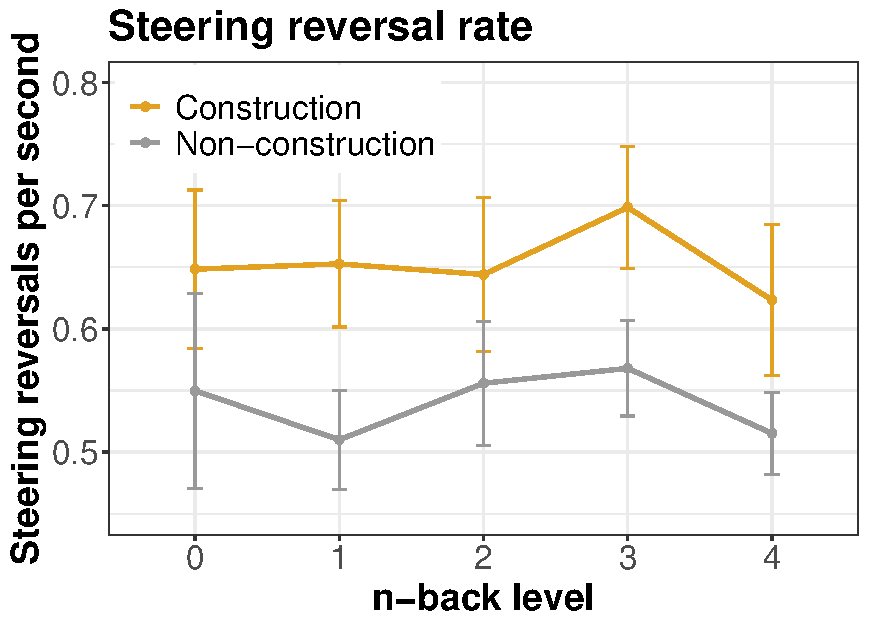
\includegraphics[width=\textwidth]{images/steering_reversal.pdf}
    \caption{Steering reversal rate (\textit{N}\ =\ 7). From \citet{Kelapanda2021}.}
    \label{fig:steering-reversal}
  \end{subfigure}
  \caption{Measures of driving performance. Bars represent standard error.}
  \label{fig:performance}
\end{figure*}

\subsection{Participants}
From the 38 individuals that participated in this experiment 16 were excluded from data analysis altogether.
8 participants were excluded because their driving behavior was not indicative of an actual attempt to perform the task.
8 additional participants were excluded due to an error in the experiment, leading to the trials being too short.
This altered the task considerably and therefore we cannot compare the behavior of these participants to others.
Thus, task error (see \citealp{DeMooij2021}) and lane deviation (see \citealp{Kelapanda2021}) were determined for 22 participants. 

For eye-tracking analysis specifically, 6 more participants were excluded as their eye-tracking data were incomplete. 
This leaves us with 16 participants for eye-tracking analysis.
Finally, for the analysis of steer reversal rate (see \citealp{Kelapanda2021}) 15 participants were excluded because of missing data, leaving 7 participants for analysis.

\subsection{Driving performance}
Let us first examine performance on the working memory task.
Figure~\ref{fig:errors} shows a positive correlation between \nback level and the proportion of errors,
confirming that the \nback task indeed gets more difficult with increasing \(n\). 
There is no effect of the construction condition, nor an interaction between \nback level and construction on the error rate.
This suggests that visuospatial demands do not impact performance on the working memory task.

Figure~\ref{fig:lane-deviation} shows the average deviation from the center of the lane.
While \nback level has no significant influence on lane deviation, there is a significant effect of construction condition.
These results indicate a positive correlation between visuospatial demands and lane deviation, and no influence of working memory load.

Figure~\ref{fig:steering-reversal} shows the rate of steering reversal.
We see an increase in steering reversals in the construction condition compared to the non-construction condition.
No significant effect of \nback level is found.

Our findings on lane deviation and steering reversals can be summarized as a negative correlation between visuospatial demands and driving performance.

\subsection{Pupil size}
% \begin{figure*}
%   \centering
%   \begin{subfigure}[b]{0.45\textwidth}
%     \centering
%     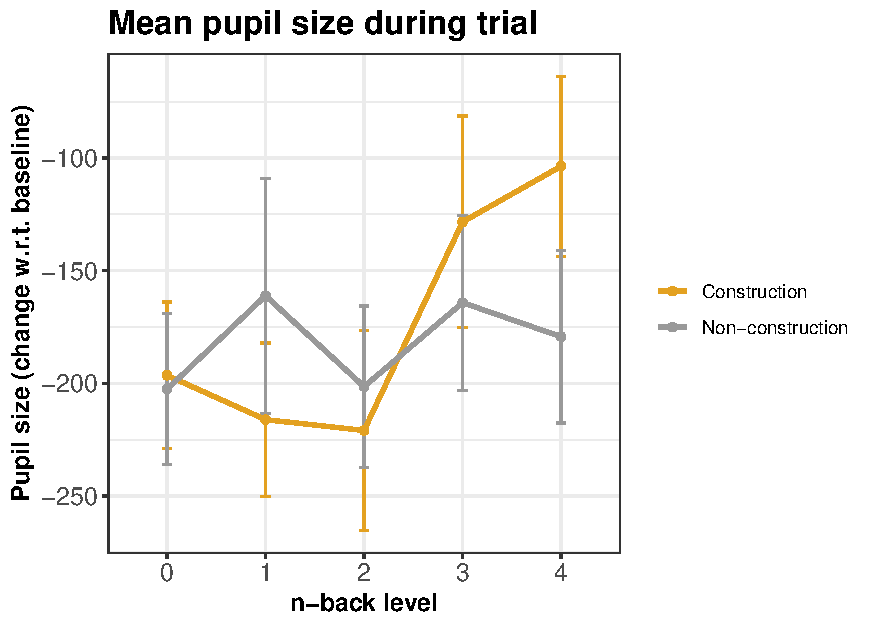
\includegraphics[width=\textwidth]{images/pupil_size_interaction.pdf}
%     \caption{Mean pupil size during trial (\textit{N}\ =\ 16).}
%     \label{fig:mean-ps}
%   \end{subfigure}
%   \hfill
%   \begin{subfigure}[b]{0.45\textwidth}
%     \centering
%     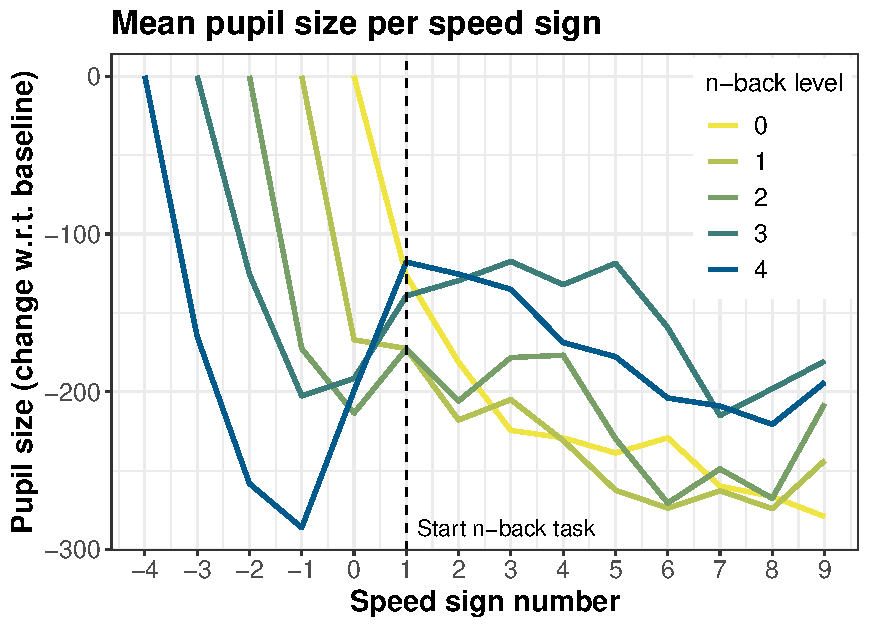
\includegraphics[width=\textwidth]{images/speed_sign_nback.pdf}
%     \caption{Mean pupil size over the period between the appearance of two speed signs (\textit{N}\ =\ 16).
%     The dashed vertical line indicates the end of the build-up phase, i.e.\ the start of the speed regulating task.}
%     \label{fig:ps-speed-sign}    
%   \end{subfigure}
%   \caption{Measures of pupil size. Bars represent standard error.}
% \end{figure*}

\begin{figure}
  \centering
  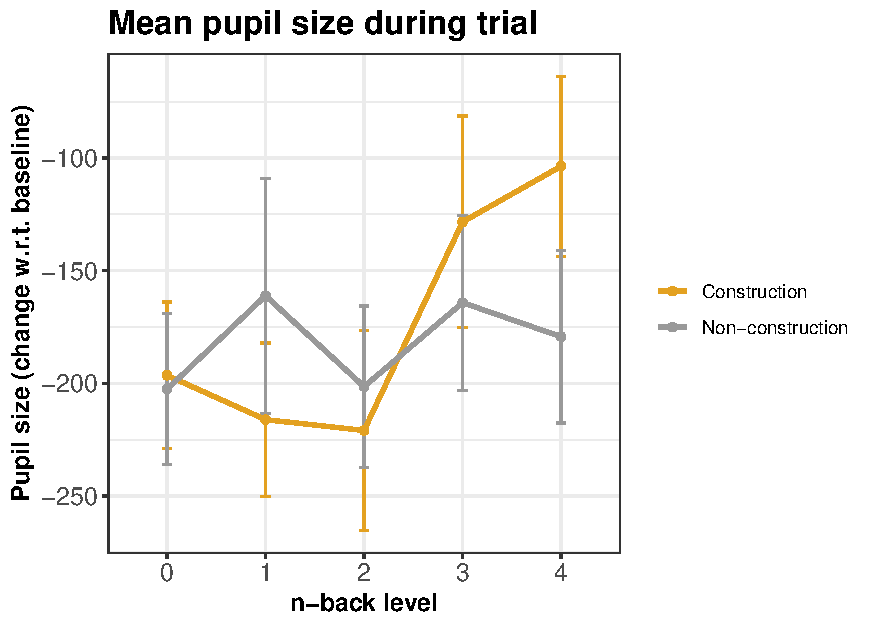
\includegraphics[width=7.5cm]{images/pupil_size_interaction.pdf}
  \caption{Mean pupil size during trial (\textit{N}\ =\ 16).}
  \label{fig:mean-ps}
\end{figure}
Figure~\ref{fig:mean-ps} shows the mean pupil size over a trial. 
There seems to be a correlation between \nback level and pupil size.
A two-way ANOVA with repeated measures confirms this effect of working memory load (WML) on pupil size [\(F(4,135)=3.09,\ p=.018\)].
No significant effect of visuospatial demands [\(F(1,135)=1.88,\ p=.17\)] or interaction between WML and visuospatial demands [\(F(4,135)=0.40,\ p=.81\)] is found.

\begin{figure}
  \centering
  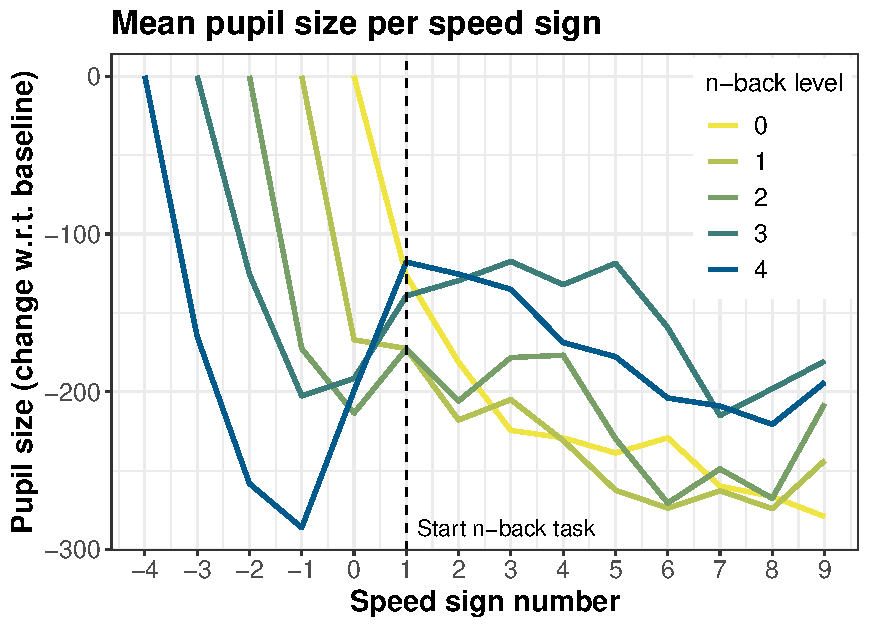
\includegraphics[width=7.5cm]{images/speed_sign_nback.pdf}
  \caption{Mean pupil size over the period between the appearance of two speed signs (\textit{N}\ =\ 16).
  The dashed vertical line indicates the end of the build-up phase, i.e.\ the start of the speed regulating task.}
  \label{fig:ps-speed-sign}    
\end{figure}

Figure~\ref{fig:ps-speed-sign} shows how the pupil size of participants changed within a trial.
It is immediately noticeable that pupil size for speed sign number \(0-n\) is equal to zero for all \nback levels.
This is explained by our definition of the baseline period (the first five seconds of a block) as speed sign number \(0-n\).
Hence, the corrected pupil size for this first ``speed sign'' is \(baseline-baseline=0\).

Looking at the changes in pupil size for \(n = 0,1\) we see a nearly continuous decrease in pupil size over the trial, indicating a low cognitive load.
In contrast, \(n=3,4\) show a larger pupil size, suggesting higher cognitive load.
Interestingly, for \(n=4\) we see a steady decrease in pupil size from the start of the \nback task. 
This implies that cognitive load decreases after the start of the 4-back task, which could be explained by the participant abandoning the task because of its difficulty. 

\subsection{Fixations on speedometer}
Figure~\ref{fig:fix-speedometer} shows the number of fixations on the speedometer as a percentage of the total number of fixations for a trial.
Like this figure suggests, there is a significant negative correlation between \nback level and fixations on the speedometer [\(F(4,135)=51.55,\ p<.001\)].
There is no effect of construction [\(F(1,135)=0.03,\ p=0.86\)] or interaction between \nback level and construction [\(F(4,135)=0.085,\ p=0.99\)]. 

\begin{figure}
  \centering
  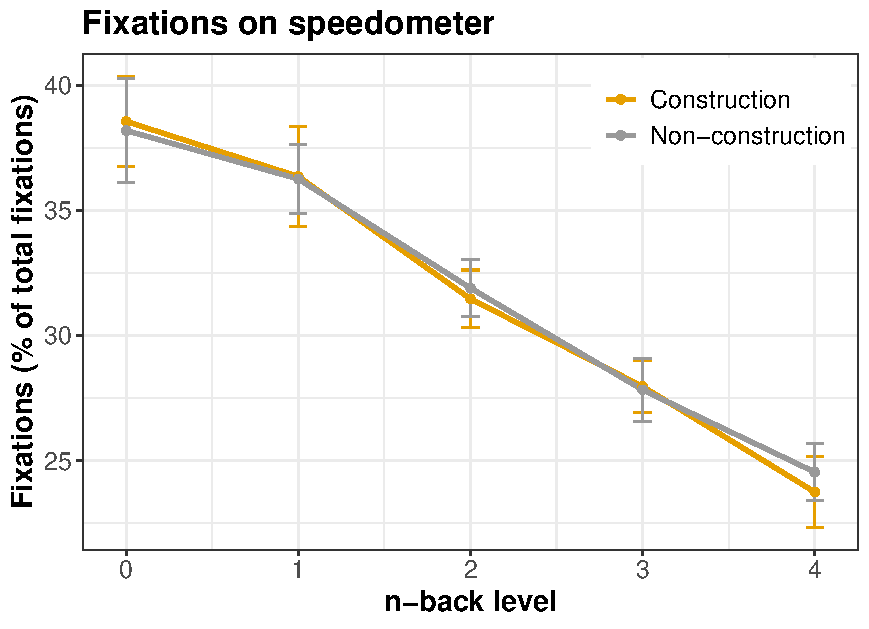
\includegraphics[width=7.5cm]{images/speedometer_interaction.pdf}
  \caption{Number of fixations on the speedometer as a percentage of the total number of fixations for that trial (\textit{N}\ =\ 16); bars represent standard error.}
  \label{fig:fix-speedometer}
\end{figure}